\chapter{Fonctions réelles et continuité}
\section{Introduction}
Dans les chapitres qui précèdent t'as déjà vu comment la notion d'\textit{ensemble} se formalise en mathématiques. Dans le cadre des fonctions réelles (d'une variable réelle) les éléments des ensembles concernés sont les nombres réels (donc tous les nombres sauf les complexes. Par exemple, \{$420, -2/5, \pi$\} $\subset \mathbb{R}.$

\begin{boxdef}[Fonction réelle]
Soient $E$  et $F$ deux sous-ensembles non vides de $\mathbb{R}$. La correspondance, qui,
à chaque nombre appartenant à $E$ associe un nombre appartenant à $F$ est appelée une \textit{fonction réelle d'une variable réelle}.
\end{boxdef}

On la note par $f$ : $E \toF$ (dit "fonction de $E$ dans $F$"). L'ensemble $E$ s'appelle alors \textit{ensemble de définition} ou \textit{ensemble de départ} et l'ensemble $F$ s'appelle \textit{ensemble d'arrivée}. Les trois éléments - $E$, $F$, et $f$, une règle qui associe des éléments de ces deux ensembles, font partie constituante d'une fonction.

\section{Ensemble de définition et image}
Chaque fois quand on définit une fonction c'est essentiel de préciser son domaine de définition. C'est important pour pouvoir appliquer certains théorèmes applicables à une fonction seulement une partie de la droite réelle. En principe, le domaine de définition est arbitraire (par exemple, on peut définir $f$ : $\mathbb{R} \to \mathbb{R}$, $f(x) = x^2$, dont le graphe serait une parabole complète mais aussi une fonction $g$ : $[0, \infty)$ → $\mathbb{R}$, $f(x) = x^2$, qui serait juste la partie "droite" de la parabole. On peut remarquer que $g$ est strictement croissante, tandis que $f$ ne l'est pas. 

Néanmoins, dans certains cas, il y a un domaine de définition maximal. Par exemple, la fonction qui associe à chaque nombre de l'ensemble de définition son inverse multiplicatif $f(x) = 1/x$ ne peut pas inclure zéro dans le domaine de définition, car zéro n'a pas d'inverse multiplicatif.

Ce n'est donc pas juste de définir $f$ : $\mathbb{R} \to \mathbb{R}$, $f(x) = \frac{1}{x}$. 

On peut pourtant définir $f$ : $\mathbb{R}^* \to \mathbb{R}$, $f(x) = \frac{1}{x}$ avec  $\mathbb{R}^* \equiv (-\infty, 0) \cup (0, \infty)$. 

En général, l'ensemble de définition doit être inclus dans l'ensemble de définition maximal.

\begin{boxdef}[Image]
Soient $E$ l'ensemble de départ et $F$ l'ensemble d'arrivée. Alors le sous-ensemble de $F$, $\{y \in R : \exists$  $x \in E$ tel que $f(x) = y\}$ est
appelé \textit{l’image} de $E$ par $f$ et on le note Im($f$). 
\end{boxdef}
Par exemple, l'image de $f(x) =$ sin($x$) est [-1, 1].

\section{Fonctions bien définies}
On a vu que les trois objets mathématiques: l'ensemble de départ $E$, l'ensemble d'arrivée $F$ et une règle $f$ sont nécessaires pour définir une fonction. Une fonction est bien définie si à \textbf{chaque} élément de $E$ il y a un et un \textbf{seul} élément de $F$ associé par le règle $f$. 

Ceci dit, un élement de $F$ peut correspondre à plusieurs éléments de $E$. 

\section{Fonctions périodiques, fonctions paires et impaires}
\begin{boxdef}[Fonction périodique]
Une fonction $f : \mathbb{R} \to \mathbb{R}$ est dite périodique de période
$T \neq 0$ si pour tout $x \in \mathbb{R} : f(x + T) = f(x)$.
\end{boxdef}
\begin{boxdef}[Fonction im.paire]
Une fonction $f$ : $E \to F$ est dite \textit{paire} si $x \in E$ implique $\text{-}x \in E$ et $f(\text{-}x) = f(x)$.
Une fonction $f$ : $E \to F$ est dite \textit{impaire} si $x \in E$ implique $\text{-}x \in E$ et $f(\text{-}x) = \text{-}f(x)$.
\end{boxdef}
La courbe d’une fonction \textit{paire} est symétrique par rapport à l’axe des ordonnées.

\section{Exemples:}
\begin{itemize}
    \item La fonction $f$ : $\mathbb{R} \to \mathbb{R}$, $f(x) = x^2$ a l'ensemble $[0, \infty)$ comme image.
    \item De même, la fonction $f$ : $[-3, \infty) \to (-5, \infty)$, $f(x) = x^2$ a l'ensemble $[0, \infty)$ comme image.
    \item La fonction $f$ : $[2, \infty) \to \mathbb{R}$, $f(x) = x^2$ a l'ensemble $[4, \infty)$ comme image.
    \item La fonction $\mathbb{R} \to \mathbb{R}$, $f(x) = \frac{1}{x}$ n'est pas bien définie car il existe un élement de l'ensemble de départ (zéro) qui n'a pas de correspondance dans l'ensemble d'arrivée.
    \item La fonction $f : \mathbb{R^*} \to \mathbb{R}$, $f(x) = \frac{1}{x}$ est bien définie.
    \item La fonction $f : \mathbb{R} \to \mathbb{R}$ définie par une règle $f(x) = \frac{1}{x}$ si $x \neq 0$ et $f(0) = 0$ est bien définie.
\end{itemize}

\section{Fonctions (strictement) croissantes et décroissantes}
\begin{boxdef}[Fonction (strictement) croissante] Une fonction $f$ : $E \to F$ est dite $croissante$ si $a, b \in E$ et
$a$ < $b$ impliquent $f(a) \leq f(b)$.
Si l'inégalité est stricte, alors la fonction est dite \textit{strictement croissante}.
\end{boxdef}
La définition d'une fonction (strictement) décroissante est analogique.

\textbf{Remarque:} Toute fonction strictement croissante est croissante.

Par exemple, la fonction constante est croissante et décroissante en même temps, mais n'est pas strictement croissante. La fonction $f$ : $[0, \frac{\pi}{2}] \to mathbb{R}$, $f(x) =$ sin($x$) est strictement croissante.


\begin{figure}[h!]
\centerline{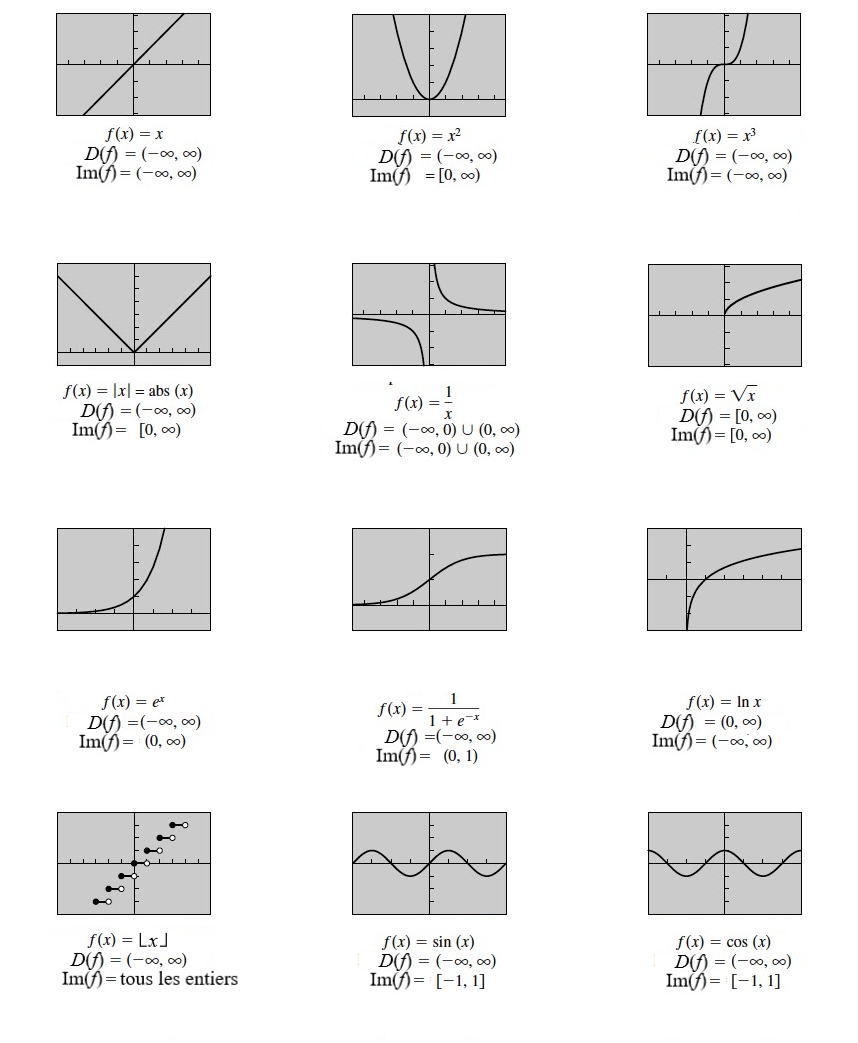
\includegraphics[scale=0.8]{content/graph.png}}
\caption{Représentation graphique de quelques fonctions usuelles.}
\label{montage}
\end{figure}

\section{Fonctions injectives, surjectives, bijectives}
On a discuté précédemment quèsaco l'ensemble de départ, l'ensemble d'arrivée et de l'image d'une fonction. Dans certaines situations (par exemple, lorsqu'on doit trouver la fonction réciproque, ou lorsqu'on change les bornes d'intégration) on s'intéresse en particulier à savoir quel est exactement le rapport entre les éléments de l'ensemble de départ et d'arrivée. 

Par exemple, pour une fonction constante genre $f$ : $\mathbb{R} \to \mathbb{R}$ , $f(x) = 1$ l'ensemble d'arrivée est $\mathbb{R}$ mais l'image est un singleton (ensemble contenant un seul élément) Im($f$) = \{1\}. 

Pour une fonction $f$ : $\mathbb{R} \to \mathbb{R}$ , $f(x) = x^2$ pour un même élément de l'ensemble d'arrivée 4, il y a deux éléments de l'ensemble de départ (à savoir 2 et -2), tandis que pour $g$ : $\mathbb{R} \to \mathbb{R}$ , $g(x) = x^3$ pour chaque élément de l'ensemble d'arrivée il y a un seul élément de l'ensemble de départ.

Pour classifier ça on utilise les termes suivants:

\begin{boxdef}[Fonction surjective]
Une fonction $f : E \to F$ est dite \textit{surjective} si tout élément $y$ de $F$ correspond à au moins un élément $x$ de $E$.
\end{boxdef}

\begin{boxdef}[Fonction injective]
 Une fonction $f : E \to F$ est dite \textit{injective} si tout élément $y$ de $F$ correspond à au plus un élément $x$ de $E$ (donc soit à un seul, soit à aucun).
\end{boxdef}

\begin{boxdef}[Fonction bijective]
Une fonction $f : E \to F$ est dite \textit{bijective} si tout élément $y$ de $F$ correspond à un seul élément $x$ de $E$ (ça veut dire injective et surjective à la fois). 
\end{boxdef}


\begin{figure}[h!]
\centerline{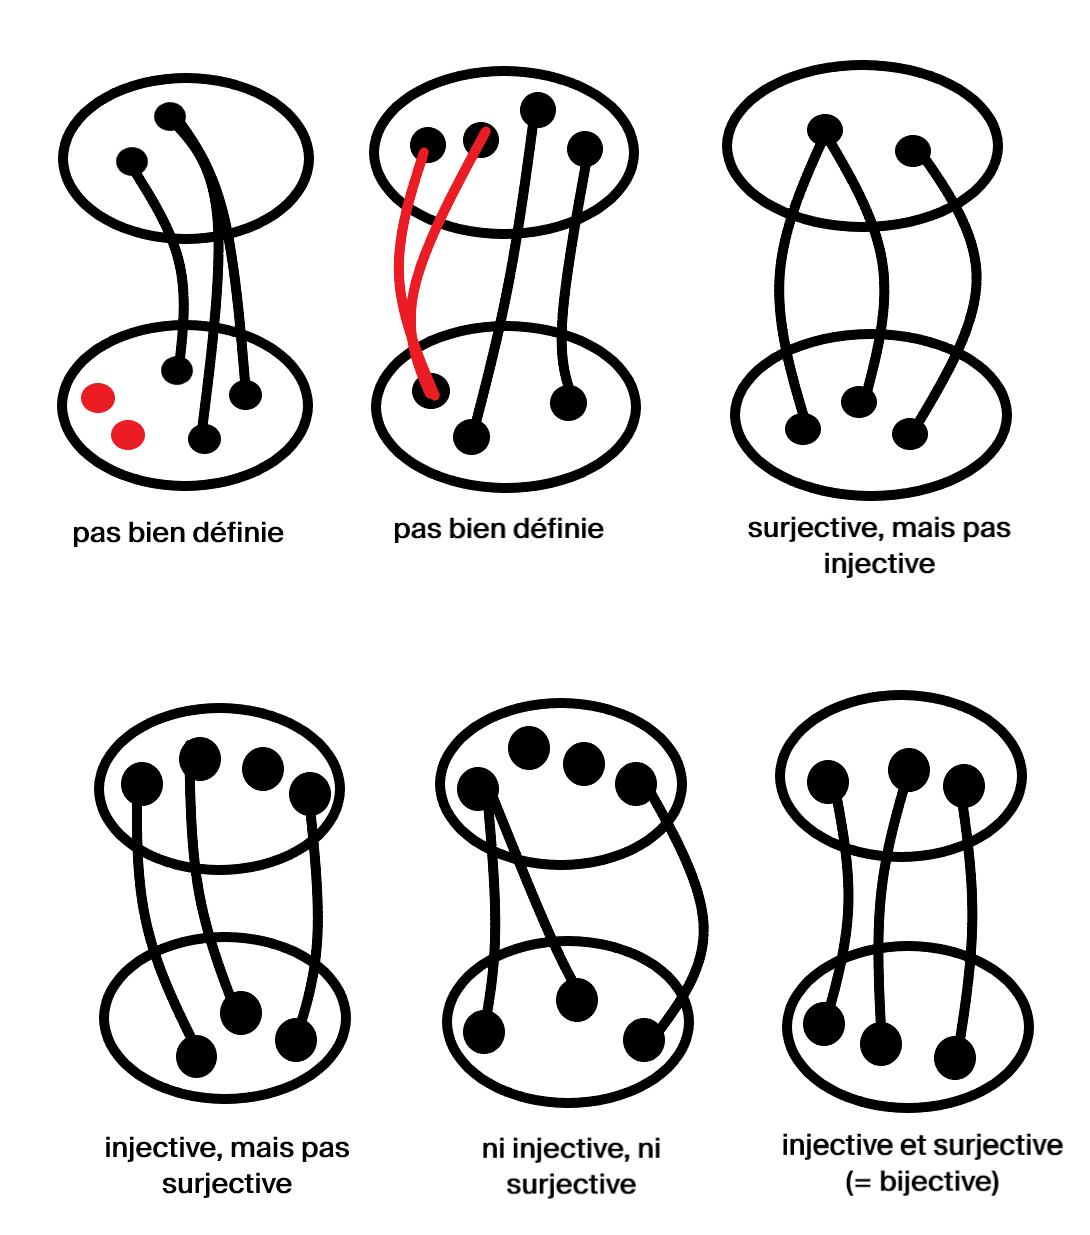
\includegraphics[scale=0.5]{content/bijectives.png}}
\caption{Représentation graphique des applications bijectives, injectives, surjectives.}
\label{sheesh}
\end{figure}

\section{Quelques fonctions réciproques :}
Lorsque la fonction $f$ : $E \to F$ est bijective, la fonction, qui, à tout élément $y$ de $F$, fait correspondre l’élément $x$ de $E$ la solution unique de l’équation
$y = f(x)$, est appelée la \textit{fonction réciproque} de $f$ et est notée $f^{\text{-}1}$.
Par exemple, 
\begin{itemize}
\item pour $f : \mathbb{R} \to \mathbb{R}$, $f(x) = x$, la réciproque est $f^{\text{-}1}$ :  $\mathbb{R} \to \mathbb{R}$, $f^{\text{-}1}(x) = x$
    \item pour $f : \mathbb{R} \to \mathbb{R}$, $f(x) = x^3$,  $f^{\text{-}1}$ :  $\mathbb{R} \to \mathbb{R}$, $f^{\text{-}1}(x) = \sqrt[3]{x}$
        \item pour $f : [0, \infty) \to [0, \infty)$, $f(x) = x^2$, $f^{\text{-}1}$ :  $[0, \infty) \to [0, \infty)$, $f^{\text{-}1}(x) = \sqrt{x}$
        \item pour $f : (\text{-}\infty, 0] \to (\text{-}\infty, 0]$, $f(x) = x^2$,  $f^{\text{-}1}$ :  $(\text{-}\infty, 0] \to (\text{-}\infty, 0]$, $f^{\text{-}1}(x) = \text{-}\sqrt{x}$
        \item pour $f : [\frac{\text{-}\pi}{2}, \frac{\pi}{2}]$ → $[\text{-}1, 1]$, $f(x) =$ sin($x$),  $f^{\text{-}1}$ :  $[\text{-}1, 1] \to [\frac{\text{-}\pi}{2}, \frac{\pi}{2}]$, $f^{\text{-}1}(x) = \text{arcsin(}x)$
         \item pour $f : [0, \pi] \to [\text{-}1, 1]$, $f(x) =$ cos($x$),  $f^{\text{-}1}$ :  $[\text{-}1, 1] \to [0, \pi]$, $f^{\text{-}1}(x) = \text{arccos(}x)$
        
\end{itemize}



\section{Graphe}

Puisque les fonctions associent à chaque $x \in D$ un unique $y = f(x) \in \mathbb{R}$, on peut les représenter par un \emph{graphe} sur un plan cartésien 2-dimensionnel, où l'on affiche les points de coordonnées $(x, f(x))$. Pour les deux fonctions $f$ et $g$ ci-dessus, on obtient les \emph{graphes} suivants~:
\begin{figure}[H]
    \centering
    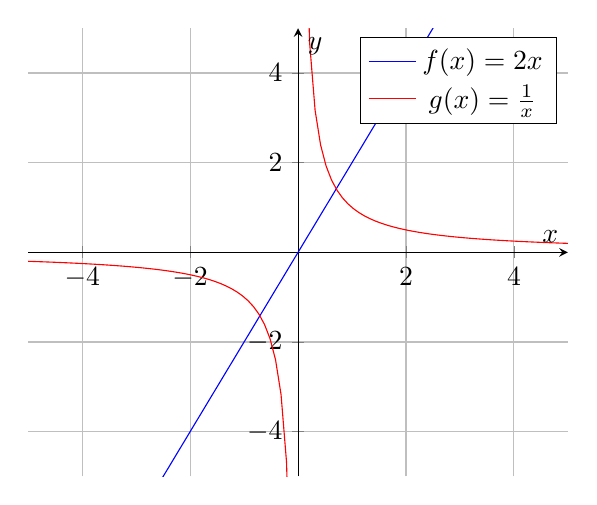
\begin{tikzpicture}
        \begin{axis}[
            xmin = -5,
            ymin = -5,
            xmax = 5,
            ymax = 5,
            xlabel = $x$,
            ylabel = $y$,
            axis lines = middle,
            grid
        ]
        
        \addplot[blue, domain=-5:5] {2 * x};
        \addlegendentry{$f(x) = 2x$};
        
        \addplot[red, domain=-5:-0.01, samples = 50] {1 / x};
        \addplot[red, domain=0.01:5, samples = 50] {1 / x};
        \addlegendentry{$g(x) = \frac{1}{x}$};
        
        \end{axis}
    \end{tikzpicture}
    \caption{Graphes des fonctions $f(x) = 2x$ et $g(x) = \frac{1}{x}$}
    \label{fig:graph_basic_functions}
\end{figure}

Gardons en tête ces deux graphes. Observons d'abord qu'ils permettent de visualiser assez facilement les propriétés de nos deux fonctions, en particulier la singularité de $g$ en 0. Il devient alors évident par le graphe qu'il est impossible de définir naturellement la division par $0$.

En outre, on pourrait dire que $f$ est \emph{plus régulière} que $g$, dans le sens où elle n'admet pas de point problématique, i.e. elle n'admet pas de saut. C'est cette intuition là que l'on cherchera à développer d'une manière plus systématique dans les prochaines sections, en cherchant ce qui fait de $f$ une "meilleure" fonction que $g$.



\section{Limite de fonction}
\subsection{Notion de convergence}
Soit $f$ une fonction réelle allant de $E$ vers $F$ deux sous-esembles de $\mathbb{R}$ et soit un point quelconque $l$ dans  $\mathbb{R}$ d'abscisse et voici son graphe :

\begin{figure}[H]
\centering \includegraphics[width = 0.55\textwidth]{assets/imgs/fonction_réelle.png}
\caption{Une fonction réelle quelconque}
\label{fig:fonction_réelle}
\end{figure}



Intéressons-nous désormais à la notion de convergence.

Cette dernière dit que si, dans l'ensemble de départ $E$, on observe que si les éléments se rapprochent toujours plus vers un autre élément $a$ dans $E$, alors on observe aussi que les images de $f$ se rapprochent aussi d'un élément $l$ dans $F$. Procédons par partie. Mais que veut dire converger ? Que veut dire se rapprocher toujours plus d'un élément ?


Imaginons que les images de la fonction $f$ convergent vers cette valeur $l$. Donc, on peut vulgariser en disant que les valeurs de $f$ se rapprochent de plus en plus de $l$. On remarque aussi que la distance entre $l$ et les valeurs de $f$, notée $\lvert f(x) - l \rvert$ tend vers $0$.


Donc, si nous choisissons une distance très petite $\epsilon$ quelconque strictement positive et qu'à partir de ce $\epsilon$ on considère les images de la fonction suffisemment proches de la limite $l$, alors on aura toujours au bout d'un moment $\lvert f(x) - l \rvert < \epsilon$.


Sauf que nous aurions pu prendre comme distance $\frac{\epsilon}{2}$ et considérer à partir de là les images de la fonctions comme proches. Dans ce cas, on peut dire que les images de la fonction sont proches si, au bout d'un moment on a $\lvert f(x) - l \rvert <\frac{\epsilon}{2}$. 


On peut prolonger le raisonnement à n'importe quelle distance $\epsilon>0$ alors on doit observer au bout d'un moment $\lvert f(x) - l \rvert < \epsilon$. 


Si l'on a cette propriété, alors on dit que les images de $f$ sont proches de la limite $l$. Donc,mathématiquement, on aura :

$$\forall \epsilon > 0, \lvert f(x) - l\rvert < \epsilon$$


Mais, nous pourrions nous poser des questions légitimes : \og comme $f$ est une fonction, quid des antécédents ? \fg , \og si oui, y a-t-il un lien entre le rapprochement des antécédents de la fonction au rappochement des images de $l$ ? \fg , \og Comment expliciter ce \og au bout d'un moment \fg ? \fg

Considérons la première question. Comme $f$ est une fonction, alors chaque antécédent doit avoir une image. Donc les images ont au moins un antécédent ce qui assure leur existance. Alors toutes les images sont aussi proches qu'on veut de la limite $l$, et il se passe la même chose pour les antécédents, les $x$ sont aussi de plus en plus proches de $a$.



Pour la deuxième question, la notion de convergence d'une fonction s'intéresse au rapprochement de $x$ vers $a$. Ce dernier est directement lié au rapprochement de $f(x)$ vers la limite $l$, car s'il  y a un rapprochement de $x$ vers $a$ et qu'il ne s'ensuit aucun rapprochement de $f(x)$ vers la limite $l$, alors par définition la fonction ne converge pas ! Comme peut l'illustrer l'image ci-dessous, on serait alors dans une telle situation.


\begin{figure}[H]
    \centering
    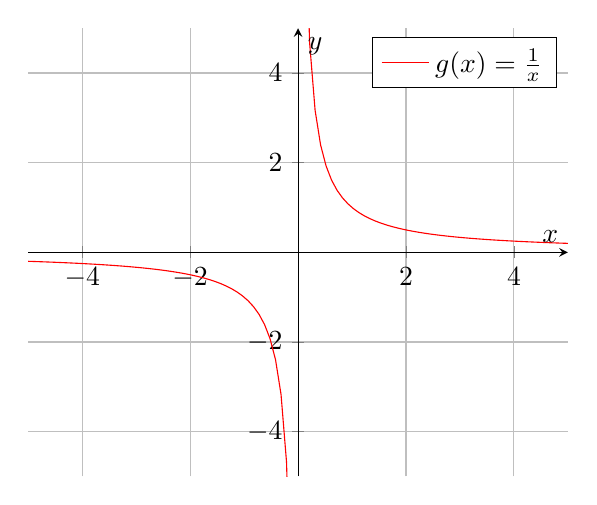
\begin{tikzpicture}
        \begin{axis}[
            xmin = -5,
            ymin = -5,
            xmax = 5,
            ymax = 5,
            xlabel = $x$,
            ylabel = $y$,
            axis lines = middle,
            grid
        ]
        
        
        \addplot[red, domain=-5:-0.01, samples = 50] {1 / x};
        \addplot[red, domain=0.01:5, samples = 50] {1 / x};
        \addlegendentry{$g(x) = \frac{1}{x}$};
        
        \end{axis}
    \end{tikzpicture}
    \caption{Graphe de $g(x) = \frac{1}{x}$. Lorsque $x$ tend vers $0$, $f(x)$ ne tend vers rien}
    \label{fig:graph_basic_functions}
\end{figure}


Pour la troisième question, ce \og au bout d'un moment \fg correspond à si $x$ est suffisemment proche de $a$, par exemple à une distance $\delta$. S'il existe ce moment, ce $\delta$, alors on doit observer que $f$ converge vers $l$.

Si l'on observe pas cela, alors la fonction diverge comme le montre la figure 4.5


Donc, si les éléments $x$ dans $E$ convergent vers un certain $a$, alors on observe que les images de $f$ se rapprochent elles aussi vers $l$. Mathématiquement, on écrit :


$$\forall \, \epsilon > 0, \, \exists \delta_{\epsilon} > 0, \, 0<\lvert x - a \rvert < \delta_{\epsilon} \, \rightarrow \lvert f(x) - l \rvert < \epsilon$$



Donc, une fonction converge vers une limite $l$ si lorsque $x$ se rapproche toujours plus vers $a$, on a alors un rapprochement toujours plus fort de $f(x)$ vers $l$.




\subsection{Limite à droite, limite à gauche}
Le Graphe \ref{fig:graph_basic_functions} de $g$ permet de voir assez facilement le comportement de la fonction autour de $0$. En effet, du côté négatif, les valeurs de $g$ sont négativement de plus en plus grandes, à mesure que l'on s'approche de 0 de la gauche. D'une manière symétrique, les valeurs de $g$ du côté positif croissent lorsque l'on s'approche de 0 de la droite. De plus, il semblerait que cette croissance soit \emph{non-bornée}, i.e. on peut trouver des valeurs arbitrairement grandes. Pour s'en convaincre, on peut écrire certaines valeurs de $g(x)$ autour de 0 du côté positif~:
\begin{table}[H]
    \centering
    \begin{tabular}{|c|c|}
        \hline
        $x$ & $g(x)$ \\
        \hline
        $0.1$ & $\frac{1}{0.1} = 10$ \\
        \hline
        $0.01$ & $\frac{1}{0.01} = 100$ \\
        \hline
        $\vdots$ & $\vdots$ \\
        \hline
        $10^{-50}$ & $10^{50}$ \\
        \hline
        $\vdots$ & $\vdots$ \\
        \hline
    \end{tabular}
    \caption{Table des valeurs de $g(x)$ quand $x \to 0$, $x > 0$}
    \label{tab:singularity_values}
\end{table}
On a alors envie d'écrire par unicité que la limite de $g(x)$ quand $x \to 0$ est $\infty$, i.e. $\displaystyle\lim_{x \to 0} g(x) = \infty$. Pourtant, lorsque l'on approche 0 du côté négatif, on a manifestement une limite différente, à savoir $-\infty$. Ainsi, que l'on approche $0$ de la droite ou de la gauche, on obtient deux résultats qui ne sont pas nécessairement égaux. Ces deux manières d'approcher un point sont matérialisées dans les notions de \emph{limite à droite} et \emph{limite à gauche} d'une fonction~: on voit à partir de notre graphe que les limites à droite et à gauche de $g$ en $0$ sont
\begin{equation}
\lim_{x \to 0^{-}} \frac{1}{x} = -\infty \quad \mathrm{ et } \quad \lim_{x \to 0^{+}} \frac{1}{x} = \infty
\end{equation}
où les notations $0^{-}$ et $0^{+}$ désignent le côté où l'on approche $0$.

Observons que les limites à droite et à gauche nous permettent de définir ce que l'on entendait par un "saut"~: une fonction n'a pas de saut en un point si les limites à droite et à gauche en ce point coïncident. Dans ce cas, on peut parler sans ambiguïté de \emph{la} limite en ce point, sans préciser le côté par lequel on approche la limite, et on la définit comme le résultat des deux limites.

Les limites de fonctions partagent de nombreuses similarités avec les limites de suites, que l'on a introduit dans le Chapitre \ref{chap:suite}. En particulier, on peut appliquer les propriétés de linéarité et le théorème des gendarmes, de la même manière que si l'on traitait avec des suites.


\subsection{Propriétés algébriques des limites de fonctions}
Comme nous l'avions vu dans les suites, nous pourrions aussi nous intéresser à la question suivante  : Si deux fonctions $f$ et $g$ convergent vers $l$ et $l'$, alors est-ce que la fonction $(f+g)$ coberge vers $l+l'$ ?


La réponse est oui et en voilà le théorème 


\begin{boxthm}[Opérations algébriques sur les fonctions : addition]
Soient $f$ et $g$ deux fonctions allant de $\mathbb{R}$ dans $\mathbb{R}$ et $a$ dans $\mathbb{R}$ et convergeant vers $l$ et $l'$ respectivement, c'est-à-dire 

$$\lim\limits_{x \rightarrow a } f(x) = l$$


Et 


$$\lim\limits_{x \rightarrow a } g(x) = l'$$


Soient $\lambda$ et $\mu $ deux réels.

Alors on a :

$$\lim\limits_{x \rightarrow a} \lambda f(x) + \mu g(x) = \lambda l + \mu l'$$
\end{boxthm}
    

 Si deux fonctions $f$ et $g$ convergent vers $l$ et $l'$, alors est-ce que la fonction $(f\cdot g)$ coberge vers $l \cdot l'$ ?

\begin{boxthm}[Opérations algébriques sur les fonctions: multiplication, inverse et quotient]
Soient $f$ et $g$ deux fonctions allant de $\mathbb{R}$ dans $\mathbb{R}$ et $a$ dans $\mathbb{R}$ et convergeant vers $l$ et $l'$ respectivement, c'est-à-dire 

$$\lim\limits_{x \rightarrow a } f(x) = l$$


Et 


$$\lim\limits_{x \rightarrow a } g(x) = l'$$


Alors on a :

$$\lim\limits_{x \rightarrow a} f(x) \cdot g(x) =  l \cdot l'$$

Si la fonction $f$ ne s'annule pas autour de $a$ et que $l \ne 0$, alors 

$$\lim\limits_{x \rightarrow a} \frac{1}{f(x)} = \frac{1}{l}$$


Et 

$$\lim\limits_{x \rightarrow a} \frac{g(x)}{f(x)} =  \frac{l'}{l}$$

\end{boxthm}



\subsection{Continuité}
En réalité, il existe plusieurs autres manières moins évidentes pour qu'une fonction admette un saut en un point. Elle peut ne pas être définie en ce point mais tout autour, ce qui cause un saut dans le domaine de définition. Il se peut aussi que la fonction soit définie en ce point, mais que les limites à droite et à gauche ne soient pas égales à cette valeur. C'est le cas de notre fonction $f$, si on change une valeur en un point, par exemple en définissant la fonction $\hat{f}(x) = \begin{cases} f(x) = 2x & \textrm{si } x \neq 1 \\ 1 & \textrm{si } x = 1 \end{cases}$.
Ainsi, 
\begin{equation}
\lim_{x \to 1} \hat{f}(x) = \lim_{x \to 1} 2x = 2 \neq \hat{f}(1) = 1
\end{equation}
et la fonction $\hat{f}$ saute lorsqu'elle arrive à 1, ce que l'on peut distinguer sur la Figure ci-dessous~:
\begin{figure}[H]
    \centering
    \begin{tikzpicture}
        \begin{axis}[
            xmin = -2,
            ymin = -5,
            xmax = 4,
            ymax = 5,
            xlabel = $x$,
            ylabel = $y$,
            axis lines = middle,
            grid,
            legend style={font=\tiny,cells={align=right}}
        ]
        
        \addplot[orange, domain=-2:0.99] {2 * x};
        \addplot[orange, domain=0.99:4] {2 * x};
        \addlegendentry{$\hat{f}(x) = \begin{cases} 2x & \textrm{si } x \neq 1 \\ 1 & \textrm{si } x = 1 \end{cases}$\\};
        
        \addplot[color=orange,fill=white,only marks,mark=*] coordinates{(1,1)};
        \draw[dotted,orange] (axis cs:1,1) -- (axis cs:1,2);
        
        \end{axis}
    \end{tikzpicture}
    \caption{Graphe de la fonction $\hat{f}$}
    \label{fig:function_jump}
\end{figure}

On définit ainsi la notion primordiale de \textbf{continuité} d'une fonction dans le fait qu'elle n'admette pas de saut, comme décrit ci-dessus~:
\begin{boxdef}[Continuité]\label{def:continuité}
Soit $f : D \to \mathbb{R}$ une fonction réelle, $a \in \mathbb{R}$ un nombre réel. On dit que $f$ est \emph{continue} en $a$ si
\begin{enumerate}
    \item Les limites à droite et à gauche existent et sont égales, i.e.
    \begin{equation}
    \lim_{x \to a^+} f(x) = \lim_{x \to a^-} f(x) \eqdef \lim_{x \to a} f(x) \in \mathbb{R}
    \end{equation}
    
    \item $f$ est définie en $a$, i.e. $a \in D$.
    
    \item La limite de $f$ en $a$ est égale à $f(a)$, i.e.
    \begin{equation}
    \lim_{x \to a} f(x) = f(a)
    \end{equation}
\end{enumerate}
On dit d'une manière similaire que $f$ est continue sur $E \subseteq D$ si $f$ est continue en tout point de $E$. (Si $D = E$, on omet généralement de mentioner $E$, et on dit simplement que $f$ est une fonction continue).
\end{boxdef}
Prenez un moment pour vous convaincre que chacun des 3 points de la définition est important dans la définition de la continuité. Le premier garantit que les voisinages à droite et à gauche du point sont au même niveau, le deuxième garantit qu'il n'y ait pas de saut horizontal dans le domaine de définition, et le dernier garantit qu'il n'y a pas de saut en le point lui-même.

La plupart des fonctions élémentaires que vous pouvez imaginer, telles que les polynômes, les fonctions trigonométriques, exponentielles, logarithmiques, etc. sont continues. De plus, la somme, le produit, le quotient et la composition de fonction continues sont des fonctions continues, ce qui permet aisément de déterminer si une fonction est continue à partir de fonction connues. Plus précisément~:
\begin{boxthm}[Propriétés des fonctions continues]
Soit $f, g$ deux fonctions réelles continues en $x \in \mathbb{R}$. Alors~:
\begin{enumerate}
    \item $f + g$ est continue en $x$.
    \item $f \cdot g$ est continue en $x$.
    \item Si $g(x) \neq 0$, $\frac{f}{g}$ est continue en $x$.
    \item Si $g$ est continue en $f(x)$, alors $g \circ f$\footnote{$g \circ f : \mathbb{R} \to \mathbb{R}$ est la fonction \emph{composée} de $f$ par $g$, définie par $(g \circ f)(x) = g(f(x))$, c'est-à-dire l'application de la fonction $f$ suivie de $g$.} est continue en $x$.
\end{enumerate}
\end{boxthm}
La démonstration du théorème est identique au théorème : opérations algébriques sur les limites de suites.
\subsection{Prolongement par continuité}
Considérons la fonction $s(x) = \frac{\sin(x)}{x}$\footnote{Culture générale~: on appelle parfois cette fonction \emph{sinus cardinal}, et on la note $\mathrm{sinc}$}, définie en tout point de $\mathbb{R}$ sauf en 0. Pour bien comprendre son comportement, prenons son graphe autour de 0~:
\begin{figure}[H]
    \centering
    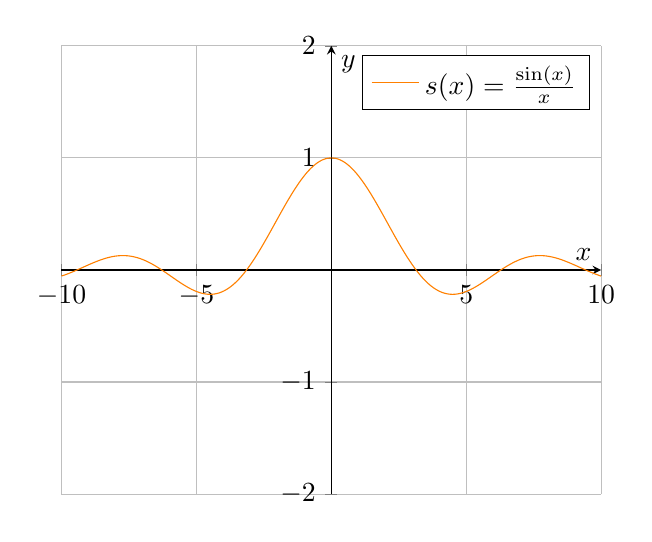
\begin{tikzpicture}
        \begin{axis}[
            xmin = -10,
            ymin = -2,
            xmax = 10,
            ymax = 2,
            xlabel = $x$,
            ylabel = $y$,
            axis lines = middle,
            grid,
            trig format plots=rad
        ]
        
        \addplot[orange, domain=-10:-0.01,samples=300] {sin(x) / x};
        \addplot[orange, domain=0.01:10,samples=300] {sin(x) / x};
        \addlegendentry{$s(x) = \frac{\sin(x)}{x}$};
        
        \end{axis}
    \end{tikzpicture}
    \caption{Graphe de la fonction $s(x) = \frac{\sin(x)}{x}$}
    \label{fig:sin_over_x}
\end{figure}
Notre fonction satisfait manifestement la première contrainte de notre Définition \ref{def:continuité}, car les limites à droite et à gauche sont égales à 1, tandis qu'elle n'est pas définie en 0. Il est possible dans ce cas de la \emph{prolonger} en une fonction continue, que l'on note avec un tilde~:
\begin{equation}
\tilde{s}(x) = \begin{cases}
s(x) = \frac{\sin(x)}{x} & \textrm{si } x \neq 0 \\
1 & \textrm{si } x = 0
\end{cases}
\end{equation}
Ainsi, $\tilde{s}$ est définie en 0, et
\begin{equation}
\lim_{x \to 0^{-}} \tilde{s}(x) = \lim_{x \to 0^{+}} \tilde{s}(x) = \lim_{x \to 0} \tilde{s}(x) = 1 = \tilde{s}(0)
\end{equation}
Donc $\tilde{s}$ est bien continue en 0 (même sur tout $\mathbb{R}$). Ce procédé de transformation d'une fonction $f$ autour d'un point problématique $a$ en une fonction continue en $a$ est appelé le \emph{prolongement par continuité} de $f$ en $a$. Notons que cette transformation est valide que si la limite existait, c'est-à-dire que le premier point doit être validé au préalable.

\begin{greybox}
\textit{Et alors ? Pourquoi c'est si important cette histoire de continuité ?}
\end{greybox}

Eh bien, la continuité a de nombreuses conséquences sur le comportement de notre fonction. Cela assure une certaine régularité locale autour d'un point, ou même plus globale si la fonction est continue sur tout son ensemble de définition. C'est ces théorèmes que l'on va aborder dans la fin de ce chapitre.

\section{Théorème de la valeur intermédiaire}
Le théorème de la valeur intermédiaire est l'un des résultats majeurs qui porte sur les fonctions continues. Il énonce que la continuité telle que nous l'avons définie respecte bien nos attentes, à savoir qu'il n'y a pas de saut dans une fonction continue sur un intervalle. Plus précisément~:
\begin{boxthm}[Théorème de la valeur intermédiaire]
Soit $f : D \to \mathbb{R}$ une fonction continue, $I = [a, b] \subseteq D$ un intervalle réel. Alors l'image de $[a, b]$ par $f$ est un intervalle, c'est-à-dire que $f$ prend toutes les valeurs entre son minimum et son maximum sur l'intervalle~:
\begin{equation}
f([a, b]) = \left[\min_{x \in [a, b]} f(x), \max_{x \in [a, b]} f(x)\right]
\end{equation}
où $f([a, b])$ désigne l'ensemble des valeurs de $f$ sur l'intervalle $[a, b]$.
\end{boxthm}
Par exemple, la fonction $h(x) = e^x + x$ est une fonction croissante et continue sur $[0, 1]$, par somme de fonction continues. Ainsi, le théorème ci-dessus implique que sur l'intervalle $[0, 1]$, $f$ atteint son minimum $h(0) = 1$, son maximum $h(1) = e + 1$, et \emph{tout nombre réel intermédiaire} entre $1$ et $e + 1$. Il nous permet e.g. d'affirmer qu'il existe un $c \in [a, b]$ tel que $h(c) = e$, car $1 \leq e \leq e + 1$.

Un cas particulier arrive lorsque $f$ est une fonction telle que $f(a) \leq 0$ et $f(b) \geq 0$. Dans ce cas, on peut affirmer qu'il existe une solution $c \in [a, b]$ à l'équation $f(c) = 0$, ce qui est l'objet du corollaire suivant~:
\begin{boxcorollary}
Soit $f : D \to \mathbb{R}$ une fonction continue sur un intervalle $I = [a, b] \subseteq D$, avec $f(a) \leq 0$ et $f(b) \geq 0$. Alors il existe $c \in [a, b]$ tel que
$f(c) = 0$.
\end{boxcorollary}
Par exemple, pour notre fonction $h$ ci-dessus, observons que
\begin{equation}
h(-1) = e^{-1} - 1 \approx -0.63 \quad \textrm{et} \quad h(0) = e^0 = 1
\end{equation}
Ainsi, on sait qu'il existe un nombre $x_0 \in ]-1, 0[$ tel que $e^{x_0} + x_0 = 0$. En fait, en rapprochant les bornes de l'intervalle, on peut approximer numériquement la valeur de $x_0$ à une précision arbitraire, et ce malgré le fait qu'il soit impossible de trouver la solution de l'équation de manière algébrique (on dit que la solution n'est pas \emph{analytique}). Ce théorème nous permet donc par une étude minutieuse de trouver le nombre de solutions d'une équation faisant intervenir des fonctions continues.

\section{Fonctions majorées, minorées, bornées}
\begin{boxdef}[Fonction majorée/minorée] Une fonction est dite \textit{majorée} (\textit{minorée}) si son image est majoré (minoré).
\end{boxdef}

Pour rappel, on dit qu'un sous-ensemble non-vide $A$ de $\mathbb{R}$ est majoré s'il existe un nombre réel $M$ tel que $x \in A$ implique $x \leq M$. De même, un sous-ensemble non-vide $B$ de $\mathbb{R}$ est minoré s'il existe un nombre réel $m$ tel que $x \in B$ implique $x \geq m$. 

\begin{boxdef}[Fonction bornée]
Une fonction majorée et minorée est dite \textit{bornée}.
\end{boxdef}

Par exemple, la fonction $f$ : $\mathbb{R} \to \mathbb{R}$, $f(x) = $ cos($x$) est bornée car son image Im($f$) = [-1, 1] est majoré et minoré (par exemple, par 1 et -1). La fonction $f : \mathbb{R^*} \to \mathbb{R}$, $f(x) = \frac{1}{x}$ n'est pas majorée ni minorée car Im($f$) = $\mathbb{R^*}$ n'a pas de majorant ni minorant. Par contre la fonction $f : (0, \infty) \to \mathbb{R}$,  $f(x) = \frac{1}{x}$ n'est pas majorée mais elle est minorée car Im($f$) = $(0, \infty)$ a un minorant, par exemple par 0.

\section{Maximum, minimum (local et global)}
\begin{boxdef}[Maximum, minimum local]
     Une fonction admet un \textit{maximum local} au point $a$ (appartenant à l'ensemble de départ) s'il existe $\delta > 0$ t.q. pour tout nombre $x$ appartenant au domaine de définition, $|x - a| < \delta$ implique $f(x) \leq f(a)$. Si, sous les mêmes conditions, $f(x) \geq f(a)$, il s'agit d'un \textit{minimum local}.
\end{boxdef}

\begin{boxdef}[Maximum, minimum global]
\textbf{Définition:} Une fonction admet un \textit{maximum global} au point $a$ (appartenant à l'ensemble de départ) si pour tout $x$ appartenant au domaine de définition, $f(x) \leq f(a)$.
\end{boxdef}

\textbf{Remarque:} Il est important dans les définitions dessus que le point $a$ appartienne au domaine de définition. Par exemple, la fonction $f$ : $(0, \infty)$ → $\mathbb{R}$, $f(x) = 1/x$, n'a pas de minimum, bien qu'elle est minorée.

\section{Théorème de min-max} \textbf{Théorème:} Soit -$ \infty < a < b < \infty$ et $f$ : $[a, b] \to \mathbb{R}$ une fonction continue.
Alors $f$ atteint son minimum et son maximum sur $[a, b]$. 

Pour une démonstration complète, je conseille de regarder la vidéo de la chaîne YouTube \textit{Øljen - Les maths en finesse} "[EM \#24] Théorème des bornes." 


(https://www.youtube.com/watch?v=LMSLj3pgYeI).

C'est une bonne méthode d'apprentissage de comprendre pourquoi chacun des hypothèses est importante:
\begin{itemize}
    \item Supposons que l'intervalle ne soit pas fermé (que ce soit $f$ : $(a, b) \to \mathbb{R}$, ou $f$ : $[a, b) \to \mathbb{R}$, ou $f$ : $(a, b] \to \mathbb{R}$ au lieu de $f$ : $[a, b] \to \mathbb{R}$.) Alors, la fonction 

    $g$ : $(0, 5] \to g(x)=1/x$ n'atteint pas son maximum et tend vers l'infini lorsque $x \to 0.$

    \item Supposons que la fonction soit discontinue. La fonction $f : [-5, 5] \to \mathbb{R}$ définie par une règle $f(x) = \frac{1}{x}$ si $x \neq 0$ et $f(0) = 0$ n'atteint pas son minimum ni son maximum.
\end{itemize}
